\part{Softwaredokumentation}
\chapter{Entwicklung}

\section{Entwicklungsumgebung}
Dieses Kapitel beschreibt das Aufsetzen der Entwicklungsumgebung für opendatahub. Voraussetzung ist eine Installation von \acs{vagrant}.
\\
\acs{vagrant} kann für alle gängigen Betriebsysteme von \url{vagrantup.com} heruntergeladen werden.


\subsection{Klonen des Git-Repository}
Der nächste Schritt ist das Klonen des Git Repositorys und starten der vagrant vm.
\begin{src}{shell}
git clone git@github.com:hsr-ba-fs15-dat/vm.git
cd vm
vagrant up
\end{src}
Wenn diese Befehle in eine *nix Konsole eingegeben werden, wird automatisch eine passende VM heruntergeladen und konfiguriert. Unter Umständen muss die Konfiguration angepasst werden. Dies kann im Config-File von puppet gemacht werden. (vm/puphpet/config.yaml)


\subsection{Initialisieren von Django}
Um mit der Entwicklung starten, folgende Befehle in der Konsole eingeben:
\begin{src}{shell}
vagrant ssh #verbindet mit der SSH Umgebung
make dev #initialisiert die venv und installiert weitere benötigte Packete
exit #ausloggen ist notwendig, damit das virtuelle environment korrekt geladen wird.
\end{src}
\subsection{PyCharm}
Wir nutzten zur Entwicklung von \acf{odh} die Entwicklungsumgebung \acs{PyCharm} für Python aus dem Hause JetBrains.
\subsection{Projekt erstellen}
Nun kann ein PyCharm Projekt erstellt werden. Dazu wählt man ``Datei $\to$ öffnen'' und wählt den opendatahub Ordner aus. Das Projekt wird erstellt. 

\subsection{Projektinterpreter}
\cref{fig:sd:vagrant-settings, fig:sd:project-interpreter-detail} beschreiben die Einstellungen, die vorgenommen werde müssen, damit alle Debugging Features funktionieren.
\begin{figure}[H]
	\centering
	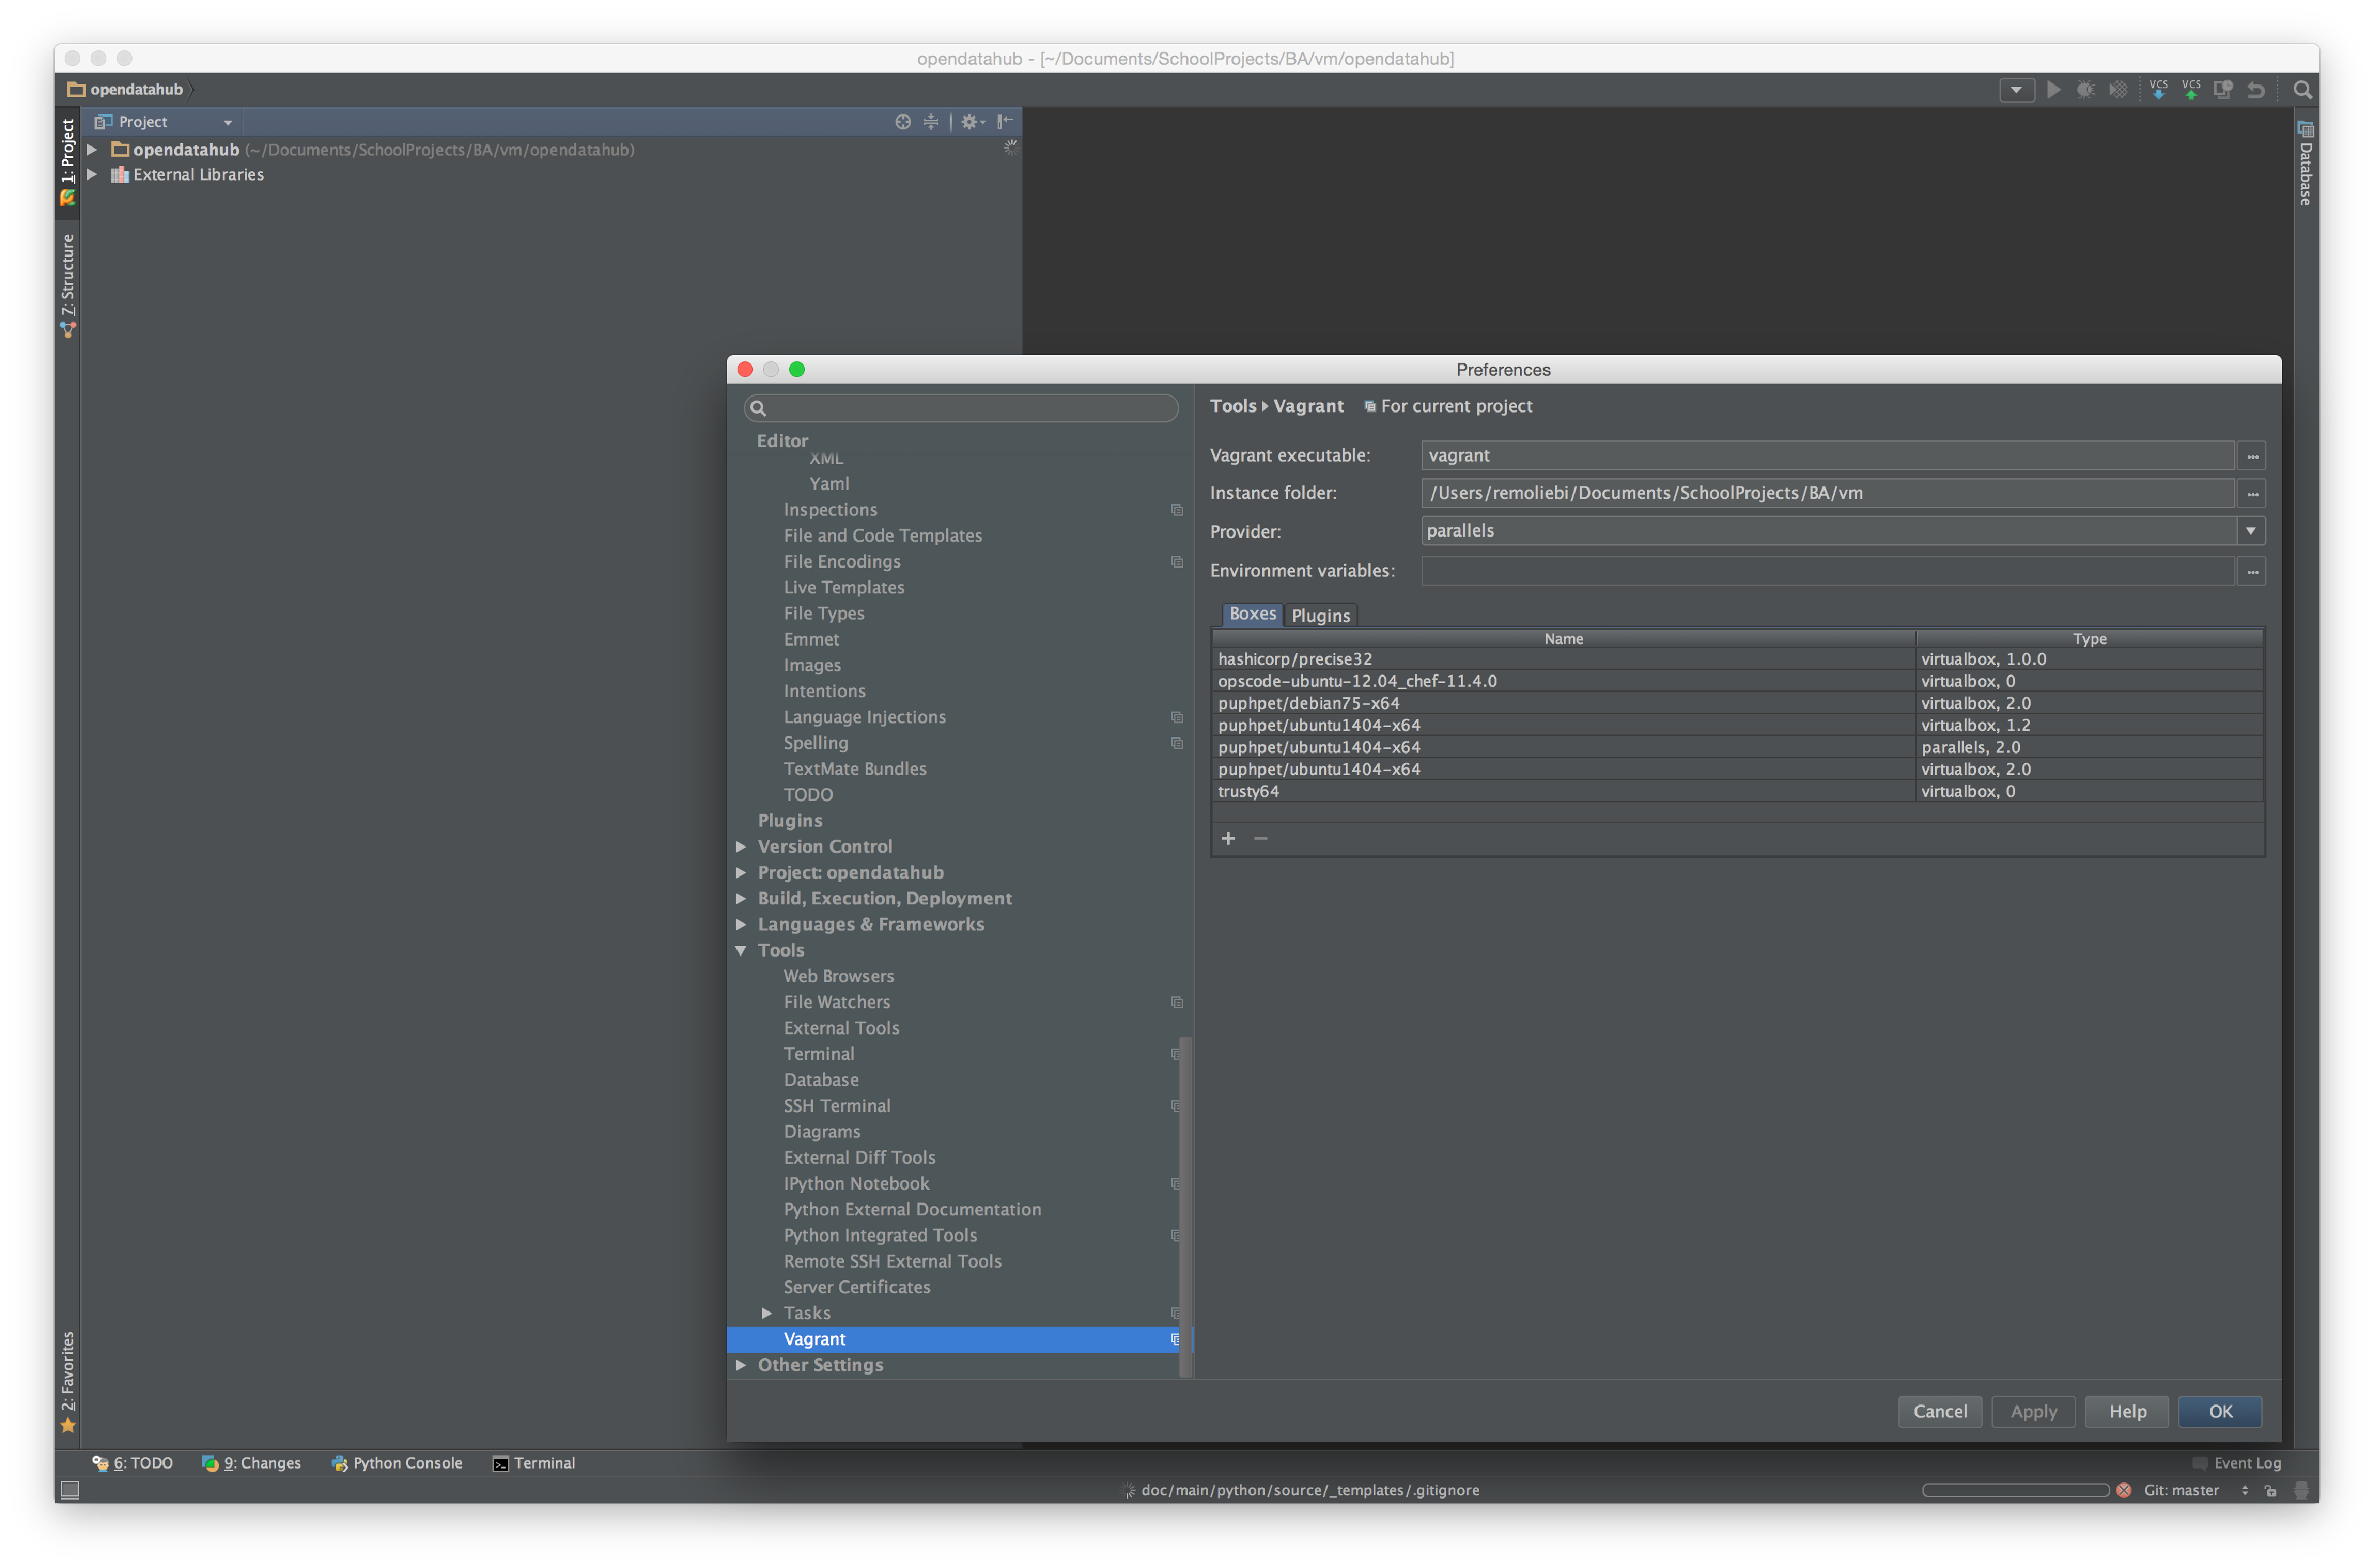
\includegraphics[width=0.8\linewidth]{fig/vagrant_settings}
	\caption{Übersicht Einstellungen: Vagrant}
	\label{fig:sd:vagrant-settings}
\end{figure}
\begin{figure}[H]
	\centering
	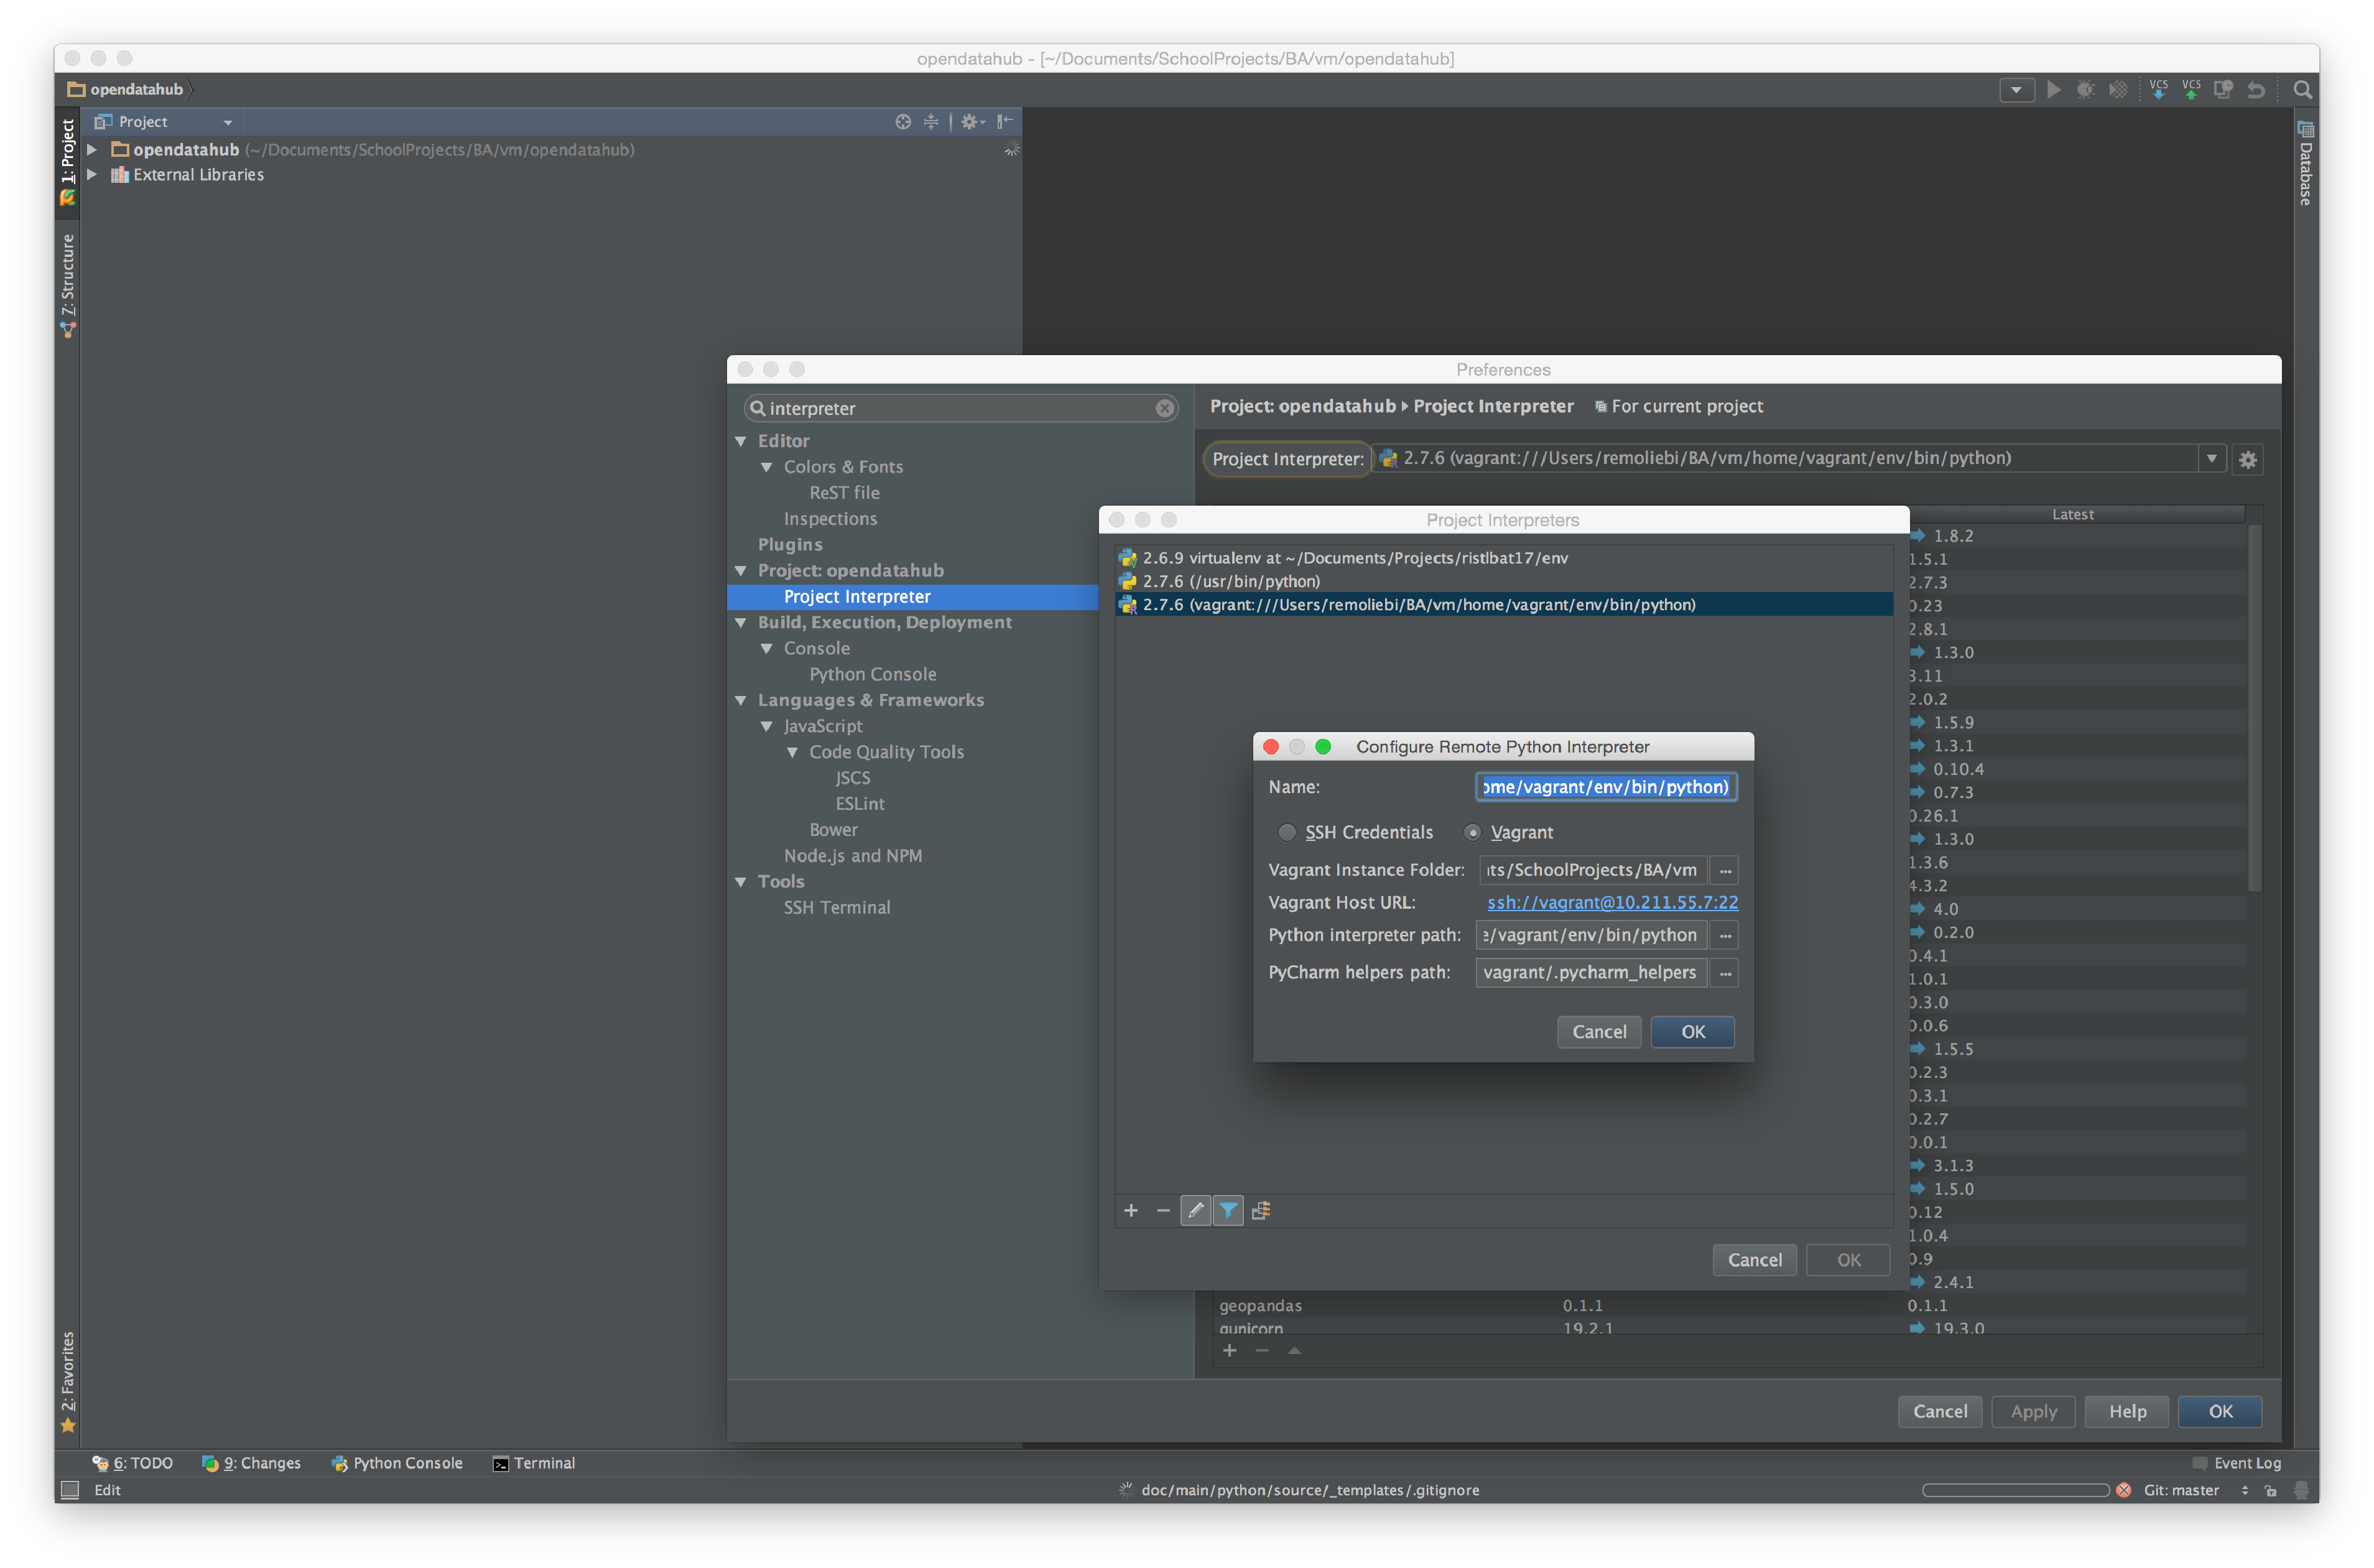
\includegraphics[width=0.8\linewidth]{fig/project_interpreter_detail}
	\caption{Übersicht Einstellungen: Projektinterpreter}
	\label{fig:sd:project-interpreter-detail}
\end{figure}


\subsection{File-Watchers}
Für die Verwendung von \ac{ts} sollte ein File-Watcher in \acs{PyCharm} eingerichtet werden. Dies wird in \cref{fig:sd:watcher-typescript} beschrieben.
\begin{figure}[H]
	\centering
	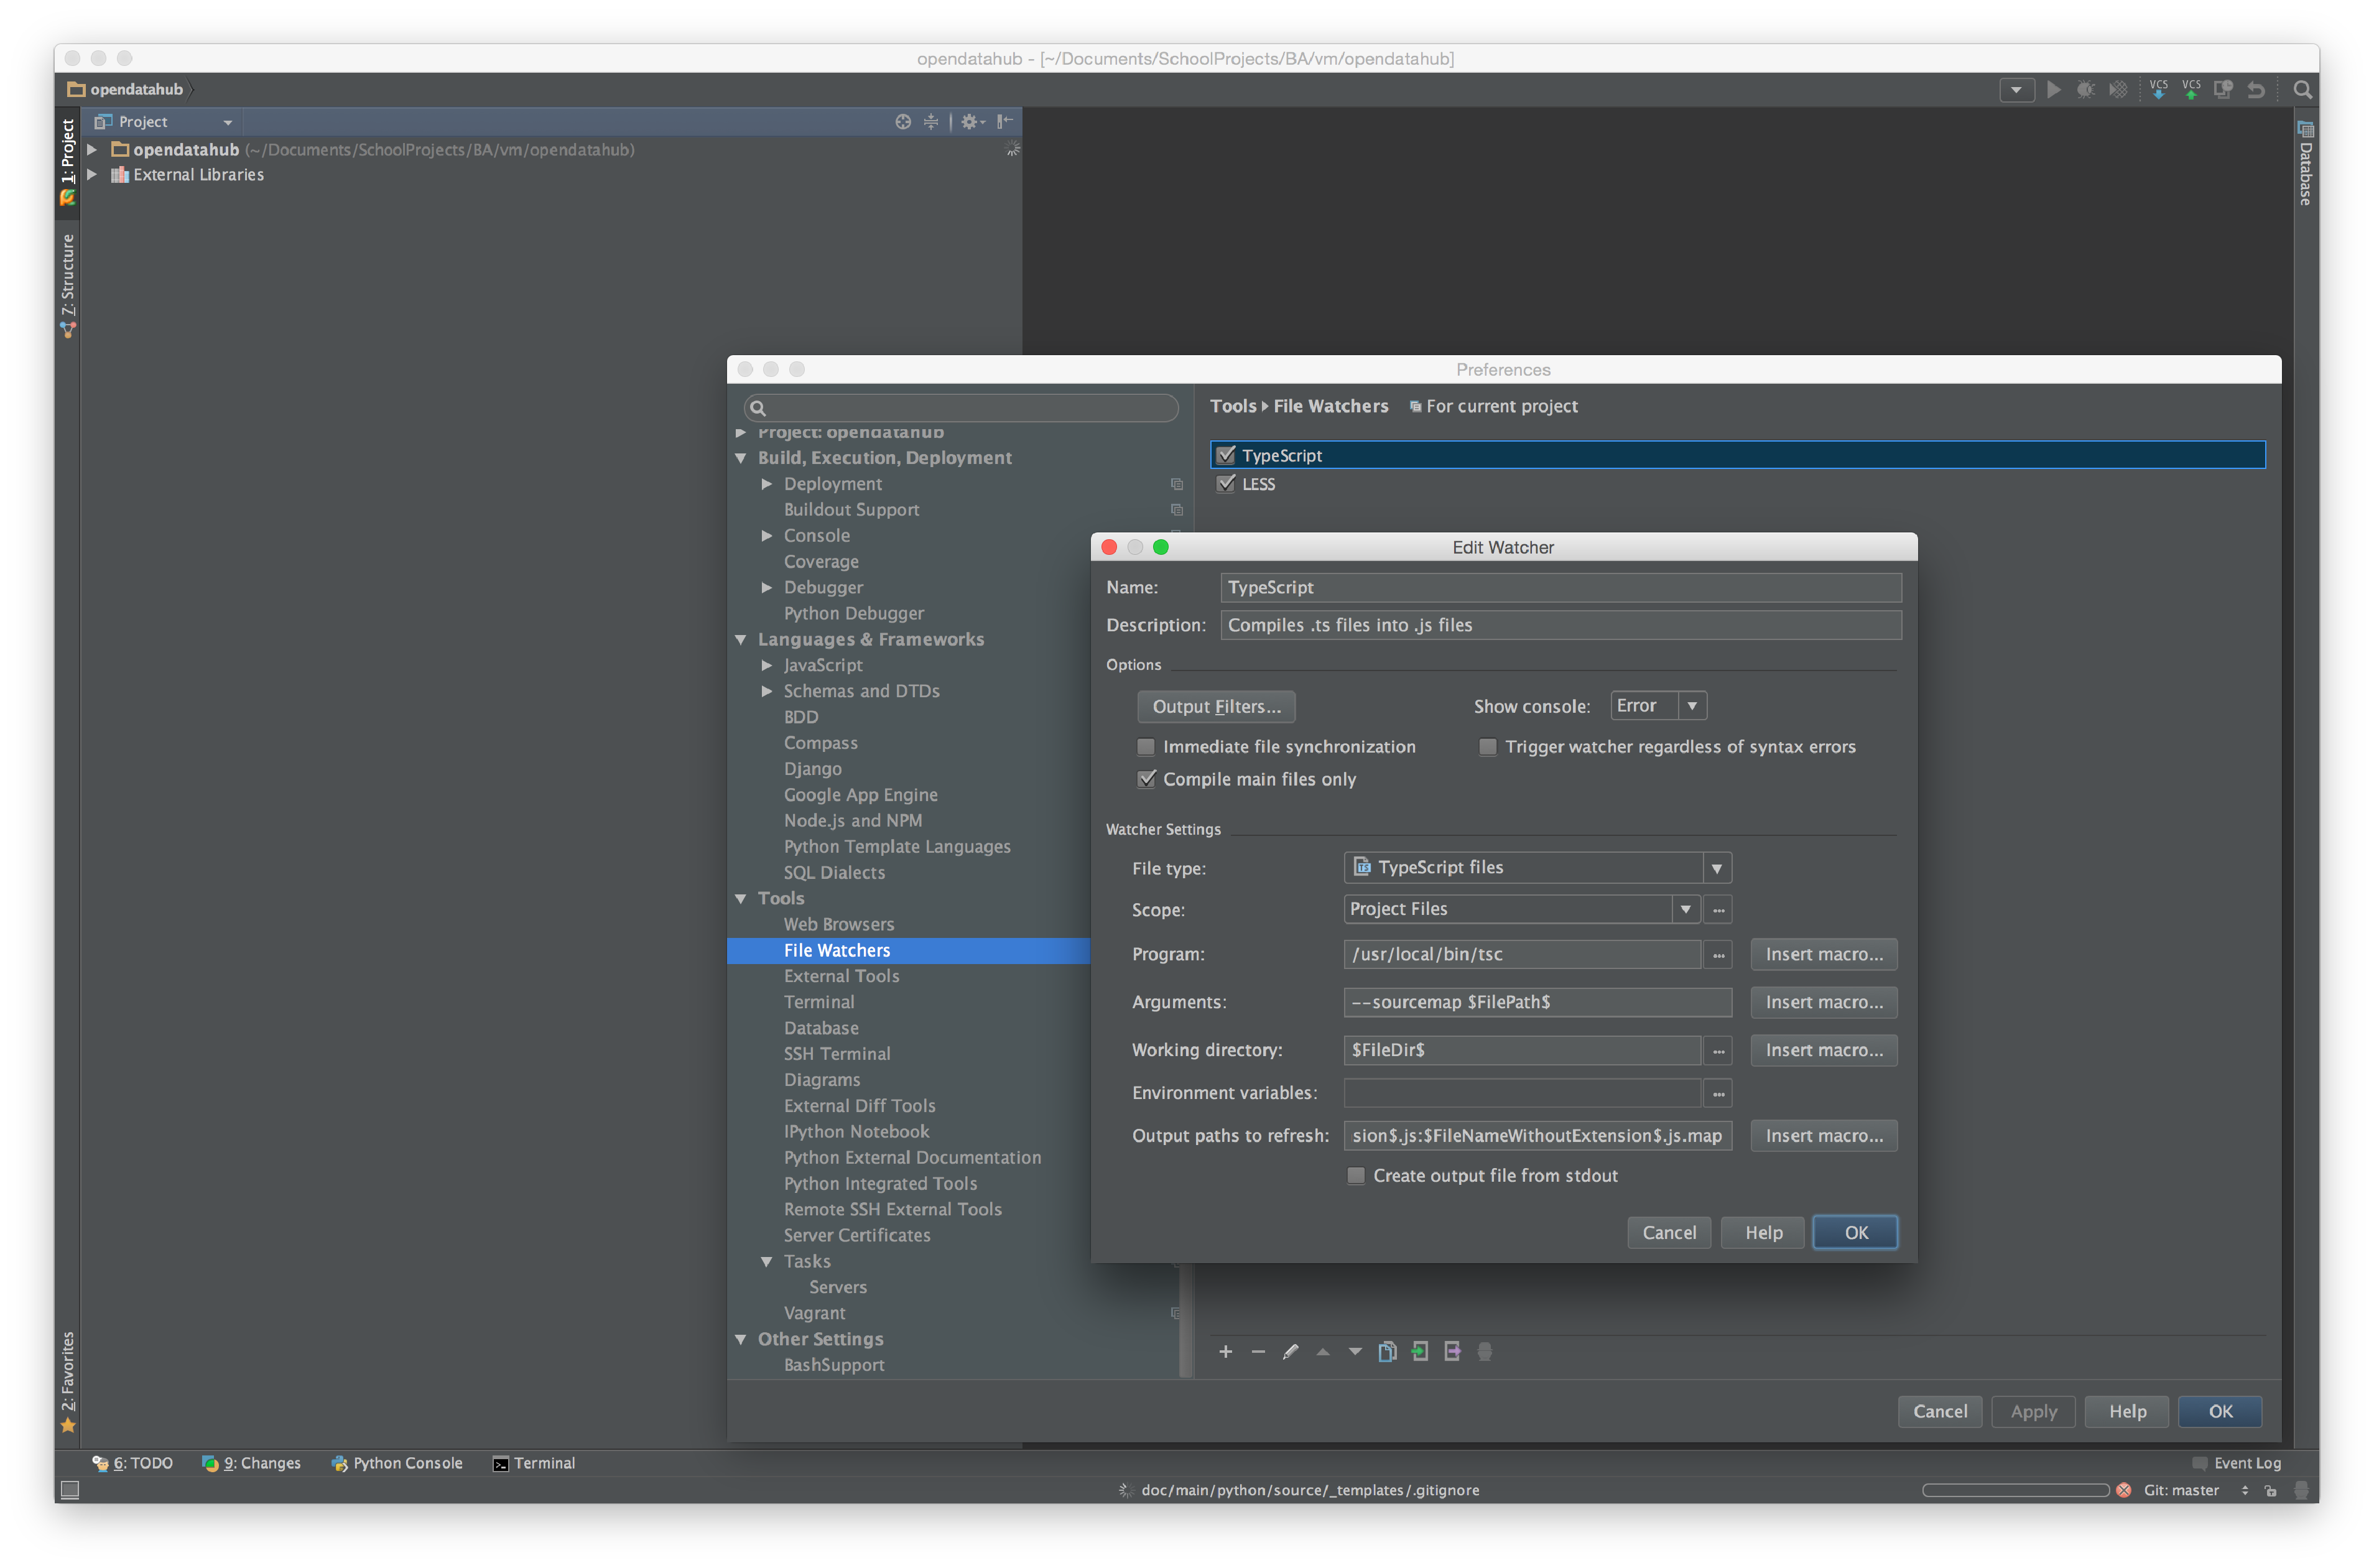
\includegraphics[width=\linewidth]{fig/watcher_typescript}
	\caption{Übersicht Einstellungen: FileWatcher: TypeScript}
	\label{fig:sd:watcher-typescript}
\end{figure}
Für die Verwendung von \ac{ts} muss tsc auf der lokalen Maschine installiert sein.

\subsection{Build}
Das ganze Projekt kann in der \ac{vm} gebuildet werden. 
\begin{src}{shell}
cd <PROJECT SOURCE>/vm
vagrant ssh #verbindet direkt in die vm
pyb -v #startet den Build-Prozess
\end{src}
\subsection{grunt}
Für die Entwicklung im FrontEnd kann ein kürzerer Weg gewählt werden \textendash Grunt.
Grunt wird wie folgt aufgeführt
\begin{src}{shell}
vagrant ssh #verbindet direkt in die vm
cd src/main/webapp # in den FrontEnd Ordner wechseln
grunt # FrontEnd Build startet.
\end{src}
Dabei werden sämtliche Less-Files, TS-Files kompiliert und geprüft.
\subsection{Deployment}
Seit der Vagrant Version 1.7 vom Dezember 2014 ist Deployment mittels Vagrant möglich. Durch den Befehl \mintinline{shell}{vagrant push} kann, je nach Konfiguration, auf Heroku, SFTP und FTP sowie durch selbstgeschriebene Kommandozeilenskripte oder Atlas deployed werden.
\\Syntaxbeispiel für einen FTP-push: \cite{vagrant-deployment}
\begin{src}{ruby}
config.push.define "ftp" do |push|
  push.host = "ftp.test.com"
  push.username = "benutzer1"
  push.password = "Passwort1"
  push.secure = false
  push.destination = "/"
  push.dir = "/"
end
\end{src}
Diese Konfiguration ist in unserem Vagrant File nicht enthalten und muss je nach FTP-Server oder Heroku Instanz konfiguriert werden.

\subsection{Tests}
Beim Build-Prozess werden Tests automatisch ausgeführt. Um nur die Python Tests auszuführen wird folgender Befehl verwendet:
\begin{src}{shell}
pyb -v django_test
\end{src}